\chapter{Technical details of Embree and ART}
\label{chap:technical_overview}

The following chapter is dedicated to the familiarization of the Embree library and the target application ART, in which Embree will be integrated. However, in this chapter, we will only consider the aspects that are relevant for our implementation. For a comprehensive overview of Embree, we would like to re-direct the reader to the Embree User Documentation \cite{embree2021Doc}, further information about ART can be found in the ART Handbook \cite{arthandbook} and the ART Scene File Reference Manual \cite{artreferencemanual} \footnote{At the time of writing this thesis, both the ART Handbook and the ART Scene File Reference Manual are still work in progress, and therefore incomplete. However, these documents are about to be completed in the near future.}.

\section{Ray Tracing with Embree}
\label{sec:embree_raytracing}

Embree follows a device concept, allowing for using the Embree API by different components of the image synthesis application without interfering with each other. An \texttt{RTCDevice} is created with the function \texttt{rtcNewDevice} and released via the function \texttt{rtcReleaseDevice}. Embree uses such device types to create further components, such as virtual scenes, which serve as the container for various scene geometry. 

\subsubsection{Scene Devices}

A scene in Embree, represented by the data type \texttt{RTCScene}, is created via the function \texttt{rtcNewScene}, to which the \texttt{RTCDevice} is passed to as an argument. It is released via the function \texttt{rtcReleaseScene}. Different geometries can be attached to the scene device by the function \texttt{rtcAttachGeometry}, which will furthermore assign a unique ID to the geometry, and detached from the scene device by the function \texttt{rtcDetachGeometry}. Once an \texttt{RTCGeometry} is attached to the \texttt{RTCScene}, it can be released via the call of the function \texttt{rtcReleaseGeometry}.

After the attachment of the complete scene geometry, the scene is committed by calling the function \texttt{rtcCommitScene} to trigger the creation of Embree's internal acceleration structures. After the invocation of this function, the individual geometries cannot be edited or manipulated.

\subsubsection{Geometries}

Geometries in Embree are represented by a \texttt{RTCGeometry} data type. These types can be created with the function \texttt{rtcNewGeometry} which takes the \texttt{RTCDevice} and an enum specifying the geometry type (e.g., triangle, quad, user defined geometry) as input parameters. In the case of the geometry is a triangle, quadrangle, or a type of curve, corresponding \emph{geometry buffers} can be created and linked to the \texttt{RTCGeometry} by invoking the function \texttt{rtcSetNewGeometryBuffer}. These buffers will store information such as vertices, indices, and surface normals of the geometry.  

To initialize a user defined geometry, one has to provide a function for calculating the bounding box for the geometry, a function for intersection testing, and another function for occlusion testings. These functions are passed to Embree as callback functions. Furthermore, the number of geometric primitives, which together compose the geometry, has to be set, and a so-called \emph{User data pointer} associated with the geometry has to be initialized. A user data pointer points to the representation of the geometry by the rendering application in memory. The user data pointer can also be associated with geometry types other than user defined geometry.
In the interior of the callback function for calculating the intersection with the user defined geometry, the original representation of the geometry can be easily retrieved via this pointer.

User data pointers are initialized with the function \texttt{rtcSetGeometryUserData}.
The passing of the various callback functions to Embree is done via invocation of the functions \texttt{rtcSetGeometryBoundsFunction}, \texttt{rtcSetGeometryIntersectFunction}, and \texttt{rtcSetGeometryOccludedFunction}.

\subsubsection{Ray Casting}

Once the \texttt{RTCDevice} and the \texttt{RTCScene} are set up, the scene geometry is attached to the \texttt{RTCScene} and the internal acceleration data structures have been built, nothing stands in the way of performing the actual ray tracing with Embree. 

\begin{listing} 
	\begin{lstlisting}[caption={The \texttt{RTCRayHit} struct. The segment of code displayed here is part of the original Embree source code.}, label={lst:rtc_ray_hit}]
	/* Combined ray/hit structure for a single ray */
	struct RTCRayHit
	{
		struct RTCRay ray;
		struct RTCHit hit;
	};
	\end{lstlisting}
\end{listing}

\begin{listing} 
	\begin{lstlisting}[caption={The \texttt{RTCRay} struct. The segment of code displayed here is part of the original Embree source code.}, label={lst:rtc_ray}]
	/* Ray structure for a single ray */
	struct RTC_ALIGN(16) RTCRay
	{
		float org_x;        // x coordinate of ray origin
		float org_y;        // y coordinate of ray origin
		float org_z;        // z coordinate of ray origin
		float tnear;        // start of ray segment
		
		float dir_x;        // x coordinate of ray direction
		float dir_y;        // y coordinate of ray direction
		float dir_z;        // z coordinate of ray direction
		float time;         // time of this ray for motion blur
		
		float tfar;         // end of ray segment (set to hit distance)
		unsigned int mask;  // ray mask
		unsigned int id;    // ray ID
		unsigned int flags; // ray flags
	};
	\end{lstlisting}
\end{listing}

\begin{listing} 
	\begin{lstlisting}[caption={The \texttt{RTCHit} struct.The segment of code displayed here is part of the original Embree source code.}, label={lst:rtc_hit}]
	/* Hit structure for a single ray */
	struct RTC_ALIGN(16) RTCHit
	{
		float Ng_x;          // x coordinate of geometry normal
		float Ng_y;          // y coordinate of geometry normal
		float Ng_z;          // z coordinate of geometry normal
		
		float u;             // barycentric u coordinate of hit
		float v;             // barycentric v coordinate of hit
		
		unsigned int primID; // primitive ID
		unsigned int geomID; // geometry ID
		unsigned int instID[RTC_MAX_INSTANCE_LEVEL_COUNT]; // instance ID
	};
	\end{lstlisting}
\end{listing}

To cast rays into a virtual scene with Embree, a per ray query intersection context, \texttt{RTCIntersectContext}, has to be set up via the function \texttt{rtcInitIntersectContext}. This structure is used for the configuration of intersection flags, among other things.
Subsequently, a \texttt{RTCRayHit} struct is declared. This struct is composed of an \texttt{RTCRay} struct, abstracting the ray that Embree uses to perform the intersection testing, and an \texttt{RTCHit} struct, in which information concerning the intersection point is stored. This information contains the surface normal, the barycentric UV coordinates of the point, and the geometry ID associated with the intersected geometry are stored.
The \texttt{RTCRay} struct stores the ray orientation and direction, so-called \texttt{tnear} and \texttt{tfar} values, indicating the boundaries of a range of possible hit distances and other information.

The \texttt{RTCRayHit}, \texttt{RTCRay} and \texttt{RTCRay} are shown in Listings \ref{lst:rtc_ray_hit}, \ref{lst:rtc_ray}, and \ref{lst:rtc_hit}.

When the target ray tracing application is generating a ray, the values of the \texttt{RTCRay} struct are updated with the ray orientation and direction. The \texttt{tnear} value is to a very small value (usually close to zero) and the \texttt{tfar} value is set to a large value. The geometry ID of the \texttt{RTCHit} struct is initialized with the macro \texttt{RTC\_INVALID\_GEOMETRY\_ID}.

After the \texttt{RTCIntersectContext} and the \texttt{RTCRayHit} structs have been successfully initialized and updated, the ray-primitive intersection testing is performed via invocation of the function \texttt{rtcIntersect1} to which the \texttt{RTCScene}, a reference to both the \texttt{RTCIntersectContext} and the \texttt{RTCRayHit} are passed as arguments. In case of a found intersection, this function will update the \texttt{tfar} value of the \texttt{RTCRay} with the closest hit distance and the geometry ID of the \texttt{RTCHit} with the geometry ID associated to the intersected geometry.

In the case of performing intersection testing between a user-defined geometry and a ray, these values must be updated manually inside the intersection function that was passed to Embree as a callback function.

When the intersecting testing procedure has finished, the geometry ID of the \texttt{RTCHit} will give insight on whether an intersection was found or not. If the value of this variable remains \texttt{RTC\_INVALID\_GEOMETRY\_ID}, one can conclude that no intersection was found. Otherwise, an intersection was found, and the \texttt{RTCRay} and \texttt{RTCHit} components of the \texttt{RTCRayHit} will provide the hit distance, the coordinates of the surface normal at the intersection point, and the UV coordinates of the intersection point.

\section{A brief introduction to ART}
\label{chap:art}

As indicated in the introductory chapter, ART considers its target audience computer graphics researchers interested in predictive rendering. Predictive rendering is a branch of the computer graphics field that is dedicated to the accurate prediction of object appearances under different viewing conditions (compare \cite{wilkie2009predictive}.) While the purpose of "conventional rendering" (to which we count the ray tracing techniques encountered in Chapter \ref{chap:fundamentals}) lies in the creation of "believable" imagery to create a certain impression to an observer, predictive rendering is concerned with the synthesis of radiometrically correct images.

Its unique predictive rendering features mentioned in the introductory chapter make ART stand apart from other rendering systems. The latest version of ART at the time of writing this thesis is 2.0.3.


\subsection{Overview of ART}
ART is composed of several UNIX-like-command line applications (hence the name Advanced Rendering \emph{Toolkit}). These applications are written in C and Objective-C.
\\

Scenes about to be rendered by ART are described in proprietary scene files. These files, with the file extension \texttt{.arm}, contain valid Objective-C code that is compiled by ART at the beginning of a rendering job.

In the following, we provide an overview of the individual applications contained in the toolkit:
\begin{description}
	% \setlength\itemsep{0.05em}
	\item[\emph{artist}] \hfil \\ This is the actual command-line application renderer, taking an ARM scene file as input and storing the raw information gathered by path tracing process in an intermediate file described in a proprietary file format.
	\item[\emph{tonemap}] \hfil \\ This tool can be used for tone-mapping the (possibly spectral) information stored in the file being created by \texttt{artist} in order to obtain viewable results.
	\item[\emph{bugblatter}] \hfil \\ This application creates difference images of two provided, same-sized images. These difference images can be useful when debugging computer graphics applications or comparing different rendering techniques.
	\item[\emph{polvis}] \hfil \\ Since ART supports rendering polarization effects by storing the amount of polarized light per pixel in each pixel of a spectral image, these polarization effects can be visualized by using this tool.
\end{description}

For our integration of Embree, the only relevant application is \texttt{artist}.
To successfully render an image with \texttt{artist} in the ARM scene file, one has to provide at least a virtual camera, the scene geometry, and so-called \emph{action sequence}. An action sequence is a user defined procedure that can be thought of as a pipeline. Other applications of the toolkit, like \texttt{tonemap} or \texttt{polvis}, can be invoked in these action sequences, too.

To execute the individual steps defined by an action sequence, which are referred to as \emph{actions}, ART makes use of a single stack data structure. During the execution of one such action, one or multiple data objects are taken off the stack, manipulated according to the action in question, and placed back on the stack. One example of such an action would be creating axis-aligned bounding boxes for each object present in the scene. Here, the scene graph object is popped from the stack, bounding boxes are calculated for each geometry, then these boxes are inserted into the scene graph. Further bounding boxes enclosing these for the geometries are calculated and inserted into the scene graph. Finally, the manipulated scene graph is pushed back to the stack.

Another noteworthy detail to mention is the ability of ART to utilize multiple available processor cores to perform a rendering job. By default, ART determines the number of available cores before the path tracing. However, a desired amount of cores to perform the rendering job can be provided by invoking

\begin{Verbatim}
$ artist foo.arm -j<n>
\end{Verbatim}

To achieve lock-free parallelism between the individual threads, the scene graph is copied, and one such copy is assigned to each thread. 
 

\subsection{Scene graph infrastructure}

Some popular rendering systems (among them Mitsuba 2 and pbrt) describe a virtual scene in the following way: A scene, abstracted by a \texttt{Scene} class object, obtains a collection of geometric shapes. These shapes are represented by a \texttt{Shape} base class, from which various geometry types are derived.

This \texttt{Shape} base class offers functions for calculating bounding boxes for the described geometry and performing intersection tests between them and a ray. This is an ideal design for Embree since these shapes can be initialized as user defined geometries. Once Embree finds an intersection with a bounding box of a particular shape, its representation in memory can be retrieved via the user data pointer and an instance function of the \texttt{Shape} class for ray-intersection testing can be called. The values of the \texttt{RTCRayHit} struct can be updated in the intersection callback function with the values.

The internal acyclic scene graph of ART diverges significantly from this design. Here, we provide an overview of different nodes in the scene graph and their functionality. The scene graph, which was assembled by ART to render the image displayed in Figure \ref{fig:csg_or}, is shown in Figure \ref{fig:scene_graph}. Table \ref{tab:nodes} displays its nodes and a brief description of their functionality and relation to other nodes. However, for reasons of brevity, we will only list nodes for which the comprehension of their functionality is important to follow the implementation described in the next chapter.
On particularity of the scene graph is that it can be utilized by every application mentioned in the previous section.

Throughout this thesis, we will refer to the subgraph rooted at the \emph{Bounding Box node}, which is a direct child of the \emph{BSP Tree node} and resembling the scene geometry as \emph{Original scene graph}. The BSP Tree node is associated with another data structure, namely the KD tree, built over the scene geometry described by the original scene graph.  

Furthermore, in the scene graph shown in Figure \ref{fig:scene_graph}, from one particular node of type \emph{Combined Attributes}, arrows with dashed lines are pointing to other nodes associated, e.g., with the BRDF of the shape represented by the child node, or nodes associated with transformation information. All of the Combined Attributes nodes have these references. For reasons of clarity, these references are shown for only one Combined Attributes node in the figure.

\begin{figure}[H]
	\centering	
	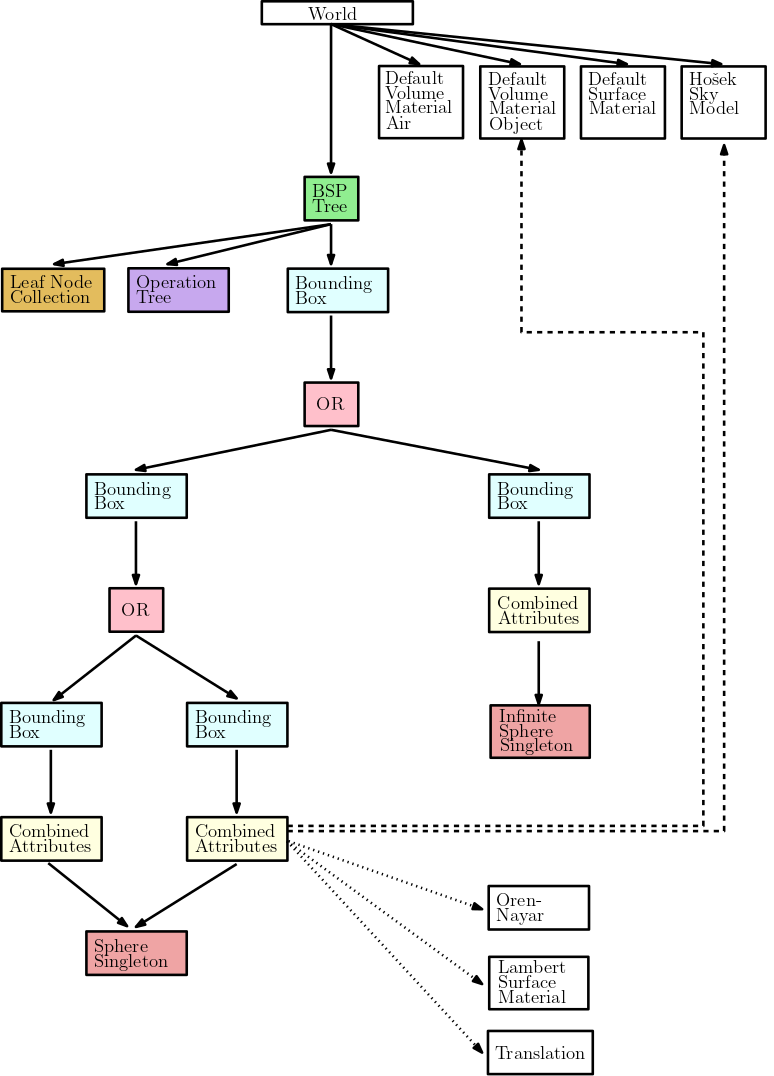
\includegraphics[width=1\linewidth]{img/2 art/scene_graph.png}
	\caption{Scene graph used to render Figure \ref{fig:csg_or}. In this graph, bounding boxes have already been inserted, and a KD tree was built over the scene. This KD tree is associated with the \emph{BSP Tree} node in the graph.} 
	\label{fig:scene_graph}
\end{figure}

\begin{table}
  \centering
  {\footnotesize
    \begin{tabular}{m{3cm}m{8cm}}
      \toprule
      Scene graph node & Function  \\
      \midrule
      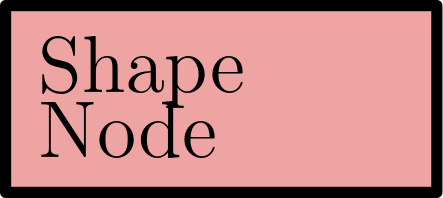
\includegraphics[scale=0.5]{img/2 art/shape_node.png} & \emph{Shape nodes} are nodes that are associated with a geometric shape, such as a sphere or a triangle. Nodes of this type are always leaf nodes. In Figure \ref{fig:scene_graph}, two such nodes are present: One representing a sphere, which is instantiated twice, and a so-called \emph{infinite sphere}, used as a skydome model.
  	  \\
      \midrule
      
\includegraphics[scale=0.5]{img/2 art/comb_attr_node.png} & \emph{Combined Attributes nodes} are superordinate to Shape nodes. They contain references to, e.g., the BRDF associated with the underlying shape and to a \emph{Transformation} node describing the transformation of the shape. In Figure \ref{fig:scene_graph}, one single Shape node is the child of two different Combined Attributes nodes. This means two instances of shape are created with different attributes.
      \\
      \midrule
    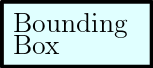
\includegraphics[scale=0.5]{img/2 art/bounding_box.png} & \emph{Bounding Box nodes}
    represent
    bounding
    boxes,
    enclosing
    the
    components
    associated with the node's children. \\
      \midrule
     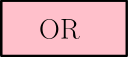
\includegraphics[scale=0.5]{img/2 art/or.png} & \emph{CSG nodes} are nodes that are associated with the Boolean set operations union (OR), difference (SUB), and intersection (AND). They have two direct child nodes. The subgraphs rooted at those child nodes represent geometries on which the set operation associated with the CSG node is applied.\\
      \midrule
     
\includegraphics[scale=0.5]{img/2 art/bsp_node.png} & The \emph{BSP Tree node} is associated with the KD tree that is built over the scene. The subgraph rooted at this node corresponds to the entire scene geometry, over which the KD tree is built.
      \\
      \bottomrule
    \end{tabular}}
  \caption{Nodes in the scene graph displayed in Figure \ref{fig:scene_graph} and their functionality.}
  \label{tab:nodes}
\end{table}


\subsection{Intersection calculation in ART}
\label{sec:art_raytracing}

A crucial part of rendering a scene in ART is the calculation of intersections between a cast ray and scene geometry and their subsequent evaluation. These intersections are calculated by traversing ART's internal KD tree.  Functionality for this traversal is abstracted in an Objective-C class called \texttt{ArnRayCaster}. Instance variables of this class store, among other information, the ray that is cast into the scene, a reference to an intersected shape, and a so-called \emph{traversal state}, which is a C struct containing references to, e.g., the surface and volume material of the intersected shape and its transformation information.

The intersections calculated by the KD tree traversal are stored in \emph{intersection lists}. An intersection list, abstracted within ART with the C struct \texttt{ArIntersectionList}. This structure is essentially a linked list, storing the individual intersections. Such an individual intersection is represented in ART by the \texttt{ArcIntersection} class, whose instance variables are a double storing the distance from the ray origin to the intersection point and references, e.g., to the intersected shape. 

There exists an alternative to the KD tree traversal in ART for calculating intersections: Namely through the traversal of the original scene graph. When considering Figure \ref{fig:scene_graph}, the original scene graph is rooted at the Bounding Box node that is a child of the BSP Tree node. The classes corresponding to the Bounding Boxes node, the CSG node, the Combined Attributes node, and the Shape node provide a function called \texttt{getIntersectionList}. When this function is called from the topmost Bounding Box node in Figure \ref{fig:scene_graph}, the function recursively calls the \texttt{getIntersectionList} functions of its children until the Shape nodes are reached, where the actual intersections are calculated. The \texttt{getIntersectionList} function of the CSG node first calls the \texttt{getIntersectionList} function of its left and right child, and then evaluates the found intersections according to the set operation this node represents.


\begin{figure}[!tbp]
	\centering
	\subfloat[Image rendered by traversing the KD Tree.]{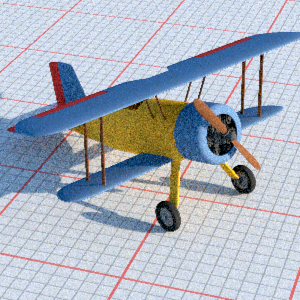
\includegraphics[width=.4\textwidth]{img/2 art/plane.png}\label{fig:render_kd_tree}}
	\hfil
	\subfloat[Image renderd by traversing the original scene graph.]{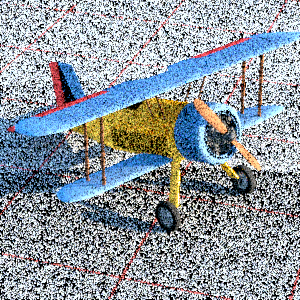
\includegraphics[width=.4\textwidth]{img/2 art/planeArtifacts.png}\label{fig:render_org_scenegraph}}
	\caption{Comparison of rendered images by traversing ART's internal KD tree and traversing the original scene graph.}
	\label{fig:org_scenegraph_comp}
\end{figure}

Although the calculation of the intersections between a ray and the scene geometry is significantly faster with this alternative procedure, since no actual acceleration data structure is traversed, traversing the original scene graph leads to visible artifacts in the resulting image. Figure \ref{fig:org_scenegraph_comp} shows a comparison between an image rendered by traversing ART's internal KD tree (Figure \ref{fig:render_kd_tree}), and the original scene graph (Figure \ref{fig:render_org_scenegraph}). The image rendered by the original scene graph traversal exhibits noticeable noise, and a black triangle is visible on the vertical stabilizer of the biplane in the image.


